% Options for packages loaded elsewhere
\PassOptionsToPackage{unicode}{hyperref}
\PassOptionsToPackage{hyphens}{url}
%
\documentclass[
]{article}
\usepackage{amsmath,amssymb}
\usepackage{lmodern}
\usepackage{iftex}
\ifPDFTeX
  \usepackage[T1]{fontenc}
  \usepackage[utf8]{inputenc}
  \usepackage{textcomp} % provide euro and other symbols
\else % if luatex or xetex
  \usepackage{unicode-math}
  \defaultfontfeatures{Scale=MatchLowercase}
  \defaultfontfeatures[\rmfamily]{Ligatures=TeX,Scale=1}
\fi
% Use upquote if available, for straight quotes in verbatim environments
\IfFileExists{upquote.sty}{\usepackage{upquote}}{}
\IfFileExists{microtype.sty}{% use microtype if available
  \usepackage[]{microtype}
  \UseMicrotypeSet[protrusion]{basicmath} % disable protrusion for tt fonts
}{}
\makeatletter
\@ifundefined{KOMAClassName}{% if non-KOMA class
  \IfFileExists{parskip.sty}{%
    \usepackage{parskip}
  }{% else
    \setlength{\parindent}{0pt}
    \setlength{\parskip}{6pt plus 2pt minus 1pt}}
}{% if KOMA class
  \KOMAoptions{parskip=half}}
\makeatother
\usepackage{xcolor}
\usepackage[margin=1in]{geometry}
\usepackage{longtable,booktabs,array}
\usepackage{calc} % for calculating minipage widths
% Correct order of tables after \paragraph or \subparagraph
\usepackage{etoolbox}
\makeatletter
\patchcmd\longtable{\par}{\if@noskipsec\mbox{}\fi\par}{}{}
\makeatother
% Allow footnotes in longtable head/foot
\IfFileExists{footnotehyper.sty}{\usepackage{footnotehyper}}{\usepackage{footnote}}
\makesavenoteenv{longtable}
\usepackage{graphicx}
\makeatletter
\def\maxwidth{\ifdim\Gin@nat@width>\linewidth\linewidth\else\Gin@nat@width\fi}
\def\maxheight{\ifdim\Gin@nat@height>\textheight\textheight\else\Gin@nat@height\fi}
\makeatother
% Scale images if necessary, so that they will not overflow the page
% margins by default, and it is still possible to overwrite the defaults
% using explicit options in \includegraphics[width, height, ...]{}
\setkeys{Gin}{width=\maxwidth,height=\maxheight,keepaspectratio}
% Set default figure placement to htbp
\makeatletter
\def\fps@figure{htbp}
\makeatother
\setlength{\emergencystretch}{3em} % prevent overfull lines
\providecommand{\tightlist}{%
  \setlength{\itemsep}{0pt}\setlength{\parskip}{0pt}}
\setcounter{secnumdepth}{5}
\usepackage{lineno}
\linenumbers
\usepackage{float}
\usepackage{booktabs}
\usepackage{longtable}
\usepackage{array}
\usepackage{multirow}
\usepackage{wrapfig}
\usepackage{colortbl}
\usepackage{pdflscape}
\usepackage{tabu}
\usepackage{threeparttable}
\usepackage{threeparttablex}
\usepackage[normalem]{ulem}
\usepackage{makecell}
\usepackage{xcolor}
\ifLuaTeX
  \usepackage{selnolig}  % disable illegal ligatures
\fi
\usepackage[]{natbib}
\bibliographystyle{plainnat}
\IfFileExists{bookmark.sty}{\usepackage{bookmark}}{\usepackage{hyperref}}
\IfFileExists{xurl.sty}{\usepackage{xurl}}{} % add URL line breaks if available
\urlstyle{same} % disable monospaced font for URLs
\hypersetup{
  pdftitle={Aquifer depletion exacerbates agricultural drought losses in the US High Plains},
  pdfauthor={Taro Mieno; Timothy Foster; Shunkei Kakimoto; Nicholas Brozovic},
  hidelinks,
  pdfcreator={LaTeX via pandoc}}

\title{Aquifer depletion exacerbates agricultural drought losses in the US High Plains}
\author{Taro Mieno\footnote{Department of Agricultural Economics, University of Nebraska Lincoln, \href{mailto:tmieno2@unl.edu}{\nolinkurl{tmieno2@unl.edu}}} \and Timothy Foster\footnote{Department of WWW, University of Manchester, \href{mailto:timothy.foster@manchester.ac.uk}{\nolinkurl{timothy.foster@manchester.ac.uk}}} \and Shunkei Kakimoto\footnote{Department of Applied Economics, University of Minnesota, \href{mailto:kakim002@umn.edu}{\nolinkurl{kakim002@umn.edu}}} \and Nicholas Brozovic\footnote{Department of Agricultural Economics, University of Nebraska Lincoln, \href{mailto:nbrozovic@nebraska.edu}{\nolinkurl{nbrozovic@nebraska.edu}}}}
\date{}

\begin{document}
\maketitle
\begin{abstract}
Aquifer depletion poses a major threat to the ability of farmers, food supply chains, and rural economies globally to use groundwater as a means of adapting to climate variability and change. Empirical research has demonstrated the large differences in drought risk exposure that exist between rainfed and irrigated croplands, but previous work commonly assumes water supply for the latter is unconstrained. In this paper, we evaluate how aquifer depletion affects the resilience of irrigated crop production to drought risk using over 30 years of data on historical corn and soybean yields, production areas, and aquifer conditions for the High Plains region in the United States. We show that aquifer depletion reduces the ability of farmers to sustain irrigated crop yields and production areas in drought years. Our findings demonstrate that drought-related production losses on irrigated croplands increase non-linearly with aquifer depletion, highlighting the need for proactive aquifer conservation interventions to support adaptation and resilience to future increases in rainfall variability under climate change.
\end{abstract}

\hypertarget{main}{%
\section{Main}\label{main}}

Groundwater is an essential input for agricultural production, providing a critical buffer against limited or variable surface water supplies for farmers in many parts of the world \citep{scanlon2023global}. Globally, agriculture's dependence on groundwater for irrigation is expected to increase in the future because of higher crop water requirements, more erratic rainfall, and more frequent and extreme drought events caused by climate change \citep{zhou2010impact, wada2013multimodel, wada2014sustainability, kreins2015quantification, florke2018water}. However, many of the world's most important aquifer systems have experienced large reductions in storage over recent decades \citep{wada2010global, famiglietti2011satellites, scanlon2012groundwater, konikow2015long, bierkens2019non}, which, if not addressed, will negatively affect the ability of farmers, food supply chains, and rural economies to use groundwater as a means of adapting to climate change.

Despite widespread alarm about the risks that aquifer depletion poses to crop productivity and food security, empirical evidence is limited about how reductions in groundwater availability will alter farmers capacity to adapt successfully to drought and rainfall variability. Most empirical studies that have assessed impacts of drought on agricultural productivity have focused primarily on rainfed production areas due to the greater exposure of rainfed agriculture to drought-related shocks \citep{schlenker2009nonlinear, lobell2014greater, schlenker2010robust, zhou2020connections, borgomeo2020impact}. Existing studies also demonstrate the importance of existing irrigated areas or future irrigation intensification to mitigate negative impacts of drought \citep{kuwayama2019estimating, zipper2016drought, zhu2022untangling, zhu2022warming, lu2020mapping, davis2019sensitivity, li2018changes}. In contrast, most research assessing impacts of aquifer depletion on resilience of irrigated farmland to drought has relied on simulation modeling \citep{foster2015well, cotterman2018groundwater, kahil2015modeling, yoon2021coupled, rad2020mod}, with more limited work that attempts to empirically evaluate change in drought-related production losses and risks on irrigated lands as a function of changing aquifer storage \citep{jain2021groundwater, suter2021depletion}.

Two pathways exist by which aquifer depletion will impact farmers' ability to access and use groundwater as a buffer against drought and rainfall variability \citep{foster2015analysis}. First, depletion increases the energy requirements and costs of pumping water, potentially making it less economically viable for farmers to satisfy crop water needs \citep{mieno2017price, bhattarai2021impact}. Second, depletion also reduces the aquifer thickness of an aquifer, lowering the aquifer's transmissivity (i.e., the potential rate of water supply to wells). This latter effect reduces the rate at which water can be pumped and applied to a field as irrigation \citep{konikow2005groundwater, foster2014modeling, hrozencik2017heterogeneous}. If the reduction in well yields is substantial - for example as would occur when a large proportion of aquifer thickness is depleted \citep{hecox2002calculation, korus2020depletion} - then a farmer may be unable to extract sufficient water to meet crop water demands, in particular during periods of limited rainfall and in the peak of the growing season when crops are most sensitive to water deficits \citep{foster2015well,rouhi2020downside}. The combined effect of these two factors could force farmers to reduce irrigation depths, resulting in greater risk of drought-related crop stress. Alternatively, or in addition, a farmer may be forced to limit irrigated area to ensure crop water demands can be met, leading to reductions in total crop production \citep{foster2014modeling, rad2020effects}. Understanding how these two responses vary as a function of aquifer conditions is crucial to guide groundwater management planning decisions, in particular given projected increases in frequency and intensity of droughts under climate change \citep{ukkola2020robust, chiang2021evidence, cook2020twenty}

In this paper, we present empirical evidence about how aquifer depletion affects farmers ability to effectively and reliably buffer crops against drought risk using data on historical crop yields, production areas, and aquifer conditions for the High Plains region in the United States. Our analysis extends previous research on the impacts of drought on agricultural production by evaluating how drought-related production losses are influenced by severity of groundwater scarcity, moving beyond prior binary comparisons of rainfed and irrigated production \citep{schlenker2009nonlinear, lobell2014greater, lu2018crop}. We also provide new empirical insights about the relative roles of extensive (i.e., irrigated area) and intensive (i.e., per-area irrigation rates) margin water use adjustments in determining drought-related production losses, which previously had only been demonstrated through theoretical modeling \citep{foster2014modeling, foster2017effects, rad2020effects}. Our findings provide important evidence of the value of preserving aquifer storage as a buffer against drought events. In doing so, our analysis adds weight to the need to improve groundwater resource conservation and sustainability to enable adaptation to climate change in groundwater-dependent agricultural systems globally \citep{jain2021groundwater, scanlon2023global}.

\hypertarget{results}{%
\section{Results}\label{results}}

\hypertarget{impact-intensive}{%
\subsection{Aquifer depletion increases sensitivity of crop yields to drought}\label{impact-intensive}}

Figure \ref{fig:yield-response} shows the estimated crop yield response to water deficit for rainfed production and groundwater-irrigated production at different levels of aquifer thickness categories for corn (panel A) and soybean (panel B)\footnote{Confidence intervals were not presented to avoid over-crowding the figures. Please see Appendix \ref{reg-conf} for estimated yield response curves with 95 percent confidence interval.}. The histogram of annual water deficit is presented at the top for each crop. In wetter years with low crop irrigation requirements (i.e., negative values of water deficit), rainfed and irrigated yields are very similar for both corn and soybean. As drought severity increases (i.e., as water deficit increases), rainfed yields of both crops decline significantly whereas irrigated yields are increasing or stable as deficit increases. This result reflects the positive benefits irrigation provides both as a buffer against precipitation variability, and as a means of raising overall yields through increased evapotranspiration and associated biomass accumulation, reductions of heat-related stressors, and other factors \citep{zhu2022untangling, li2020quantifying}.

We now focus on comparing yield response to water deficit among the three aquifer thickness categories (all irrigated). First, for water deficits above around 400mm, yield changes become negative for counties with the lowest levels of aquifer thickness (i.e., 1st quantile in Figure \ref{fig:yield-response}). This likely reflects the restrictions that lower aquifer thickness and associated reductions in well yields place on farmers' ability to fully meet crop water requirements during periods of more severe or extended precipitation deficits \citetext{\citealp[\citet{foster2014modeling}]{rad2020effects}; \citealp{hrozencik2017heterogeneous}}. However, yield gradually increases as water deficit increases for counties with the highest level of aquifer thickness.

Figure \ref{fig:yield-dif} shows the difference in yield of the second and third (highest) aquifer quantiles relative to the first (lowest) quantile with the 95 percent confidence interval for corn an soybean. For corn, in years with water deficit higher than about 800 mm, the highest aquifer thickness group has statistically significantly higher yields than the lowest aquifer thickness group. At an extreme water deficit level of 950 mm (average water deficit in 2012, the most extreme drought in our historical record), the difference is 1.15 tonne/ha. At low water deficits (below 200mm), counties with the highest levels of aquifer thickness (i.e., 3rd quantile in Figure \ref{fig:yield-response}) experience statistically lower yields than counties with the lowest level of aquifer thickness (1st quantile). This counter-intuitive result may be due to the increased possibility of over-irrigation in regions with high aquifer thickness and well capacities \citep{foster2019assessing, gibson2017case, gibson2019benchmarking}. Unlike corn, soybean yields are not statistically distinguishable among the three aquifer thickness groups. This is likely because soybean is not as water demanding as corn and even the counties the lowest aquifer thickness level can catch up with water demand in severe drought years just as well as counties with higher aquifer thickness levels.

\begin{figure}[H]

{\centering 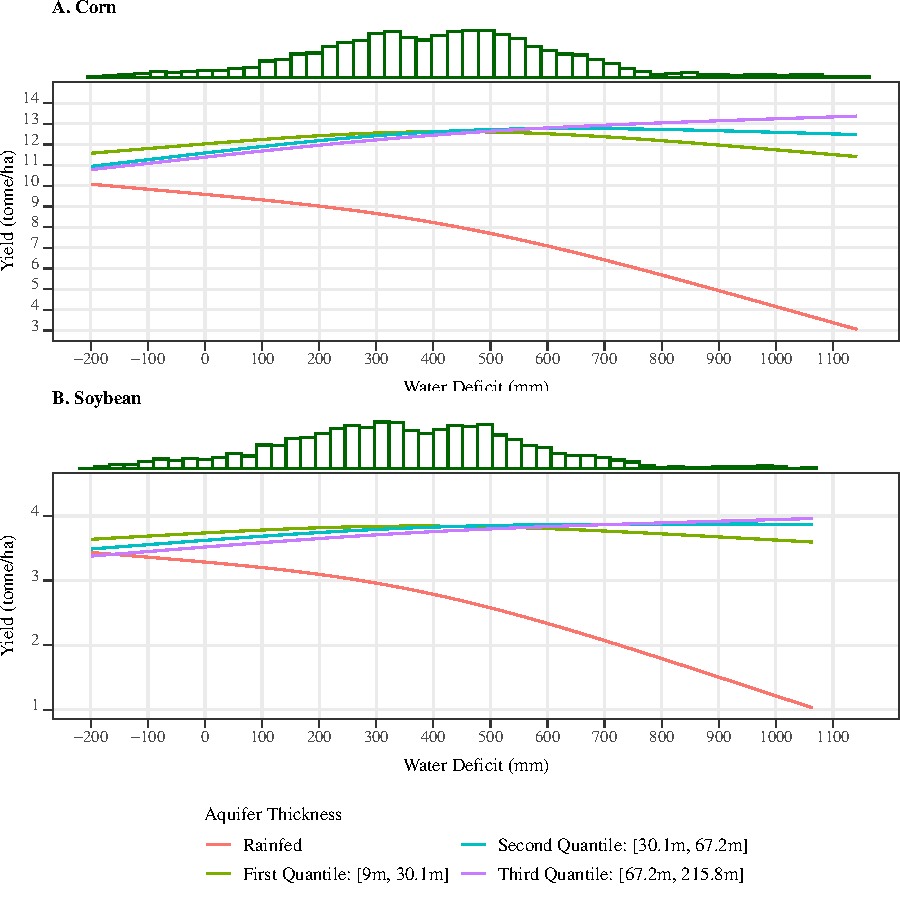
\includegraphics[width=6.5in,]{Figures/g_yield_intensive} 

}

\caption{The impact of water deficit and aquifer thickness on rainfed and irrigated per-area irrigated yields of corn and soybean in US High Plains}\label{fig:yield-response}
\end{figure}

\begin{figure}[H]

{\centering 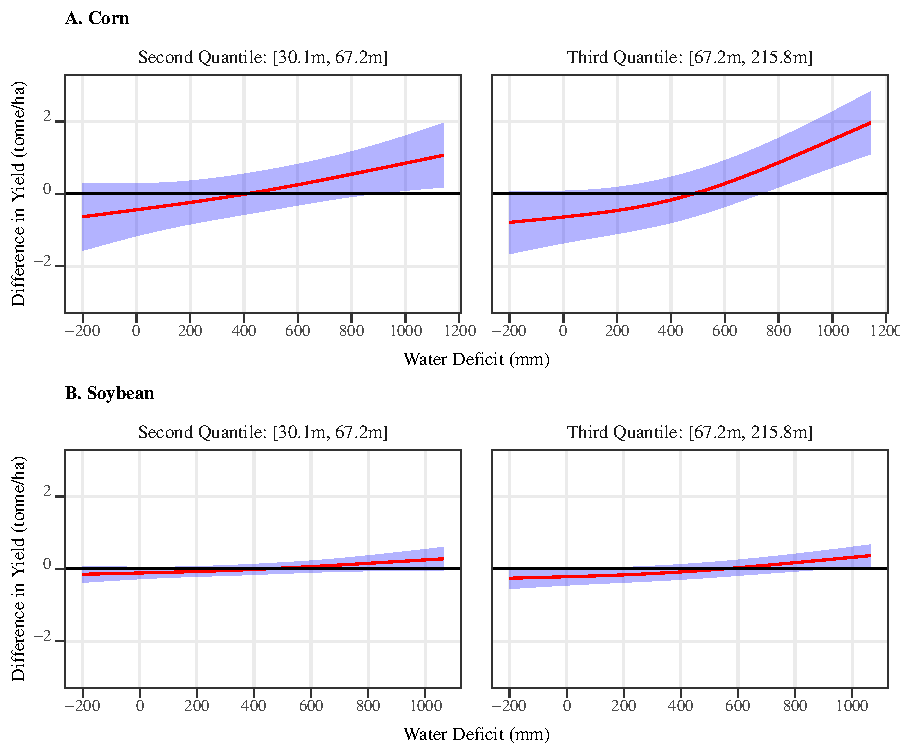
\includegraphics[width=6in,]{Figures/g_ir_yield_dif} 

}

\caption{The difference in yield for the counties with the second and third (highest) aquifer thickness groups relative to the first (lowest) aquifer thickness group.}\label{fig:yield-dif}
\end{figure}

\hypertarget{impact-share}{%
\subsection{Aquifer depletion substantially reduces the share of agricultural land under irrigation}\label{impact-share}}

While aquifer thickness has a statistically significant impact on per-area irrigated crop yields in drought conditions (more than 800mm water deficit), the magnitude of the yield impact is small when compared to differences between irrigated and rainfed production. One explanation for this result is that farmers may choose to retain a smaller proportion of land in irrigated production, so that limited groundwater pumping capacity can be used to adequately buffer crops against drought on land that remains under irrigation. Reductions in irrigated areas as an aquifer is depleted have been demonstrated theoretically \citep{rad2020effects, foster2014modeling, hrozencik2017heterogeneous, deines2020transitions}, but there has been little empirical research on farmers' irrigated area choices or how these are affected by combinations of drought exposure and groundwater scarcity.

Figure \ref{fig:ir-share} shows the estimated relationship between aquifer thickness and the share of production area that is irrigated for corn and soybean after accounting for spatio-temporal variations in drought risk exposure across the aquifer. Figure \ref{fig:ir-share} demonstrates clearly that aquifer thickness has large and significant impacts on the share of irrigated production, in particular for corn. As aquifer thickness declines, the share of irrigated acres for corn decreases from around 0.86 (86\%) for an average county-level aquifer thickness of 150m to 0.63 (63\%) for an average county-level aquifer thickness of 12m. Reductions in the share of production area under irrigation is also evident for soybean, although the effect is less pronounced than for corn potentially due to soybean's lower water requirements and susceptibility to drought than corn \citep{zipper2016drought, ruess2022irrigation}.

\begin{figure}[H]

{\centering 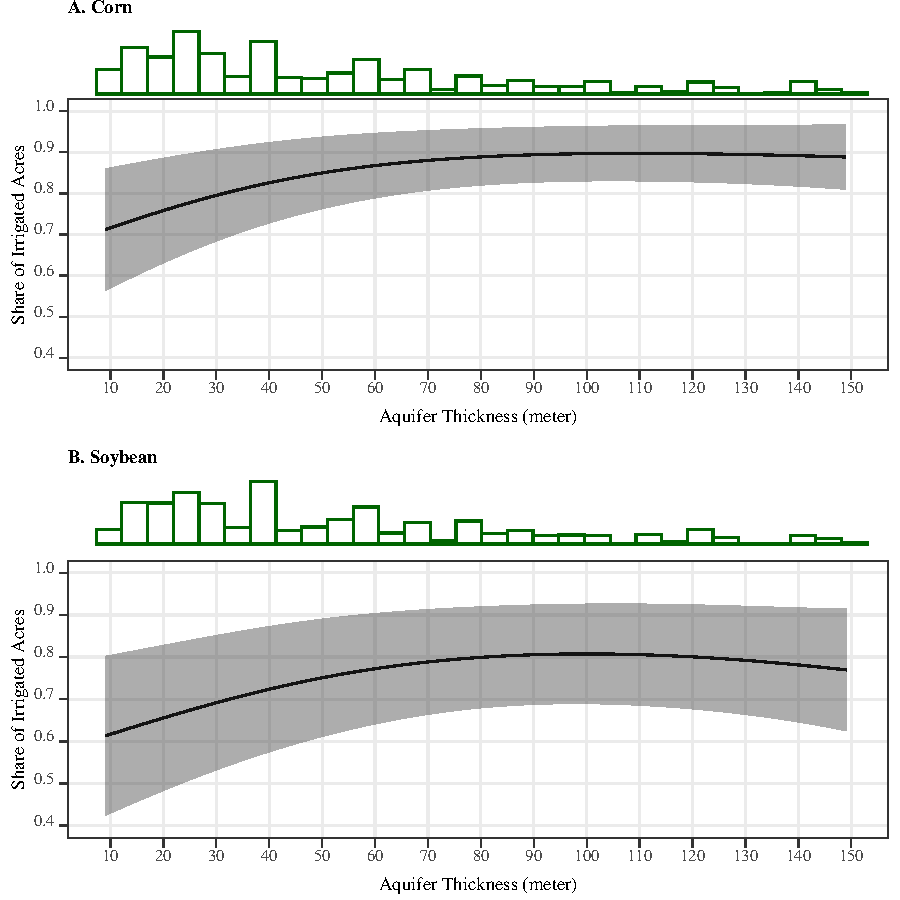
\includegraphics[width=5in,]{Figures/g_share} 

}

\caption{The impact of aquifer thickness on the share of agricultural production under irrigation for corn and soybean in the US High Plains (Note: shaded area represents 95 percent confidence interval)}\label{fig:ir-share}
\end{figure}

\hypertarget{aquifer-depletion-increases-overall-drought-related-production-losses-by-up-to-25j}{%
\subsection{\texorpdfstring{Aquifer depletion increases overall drought-related production losses by up to \(25\%\)j}{Aquifer depletion increases overall drought-related production losses by up to 25\textbackslash\%j}}\label{aquifer-depletion-increases-overall-drought-related-production-losses-by-up-to-25j}}

The overall effects of aquifer depletion on drought-related production losses is a function of both per-area irrigated yield and irrigated area changes highlighted in Sections \ref{impact-intensive} and \ref{impact-share}. Combining both responses, Figure \ref{fig:tot-impact} shows the relationship between water deficit and average per-area production (weighted-average of irrigated and rainfed yields, where weights are production area shares) for corn and soybean at thee values of aquifer thickness: 10, 50, 90, and 130 meters\footnote{Confidence intervals were not presented to avoid over-crowding the figures. Please see Appendix \ref{reg-conf} for estimated average yield response curves with 95 percent confidence interval.}. While you can see similar trends as presented in Figure \ref{fig:yield-response}, the difference in production loss caused by high water deficits among the aquifer thickness levels are much more pronounced mainly dues to lower irrigated area for lower aquifer thickness level (rainfed production has a larger share).

Figure \ref{fig:dif-tot-impact} shows the difference in average per-area production of the 50m, 90m, and 130m aquifer thickness levels relative to 10m with the 95 percent confidence interval for corn and soybean. For corn, aquifer thickness does not have a significant impact on productivity when precipitation deficits are small (less than around 200mm and 300mm for 50m and 90m aquifer thickness, respectively). However, beyond this threshold, higher levels of water deficit result in noticeable and statistically significant reductions to average corn production. This reflects the combination of lower irrigated yields under drought conditions, and, more importantly, reduced overall productivity due to smaller share of land under irrigation in areas and years where aquifer thickness is lower. Similar effects are also observed for soybean, although reductions in average production only occur at a higher deficit threshold (i.e.~greater than around 800mm) and are smaller in overall magnitude. For example, for a seasonal water deficit of 950mm (average water deficit in 2012, the most extreme drought in our historical record), average corn and soybean productivity are about 25\% and 15\% lower, respectively, when differentiating between areas with the highest (3rd quantile) and lowest (1st quantile) aquifer thickness.

Further, notice that the impact of aquifer thickness on the decline in average per-area production is highly non-linear at high seasonal water deficits. Going from 130m aquifer thickness to 90m (decline of 40m) would result in merely 0.1 tonne/ha of production loss for corn. This negligible difference in average yield from the decline is due to the insensitivity of the share of irrigated acres to aquifer thickness when the aquifer thickness level is high.
Going from 90m aquifer thickness to 50m (decline of 40m) would result in 0.42 tonne/ha of production loss for corn. However, going from 50m aquifer thickness to 10m (decline of 40m) would result in 2.18 tonne/ha of production loss for corn. That is, the same degree of decline is much more damaging when the decline is from a low aquifer thickness level than a higher aquifer thickness level. This is primarily due to the non-linear impact of aquifer thickness on the share of irrigated corn acres as shown in Figure \ref{fig:ir-share}. When aquifer thickness level is high enough (e.g., 100m), a small decline does not reduce the share of irrigated acres. However, when aquifer thickness level is low (e.g., 40m), a small decline does reduce the share of irrigated acres.

\begin{figure}[H]

{\centering 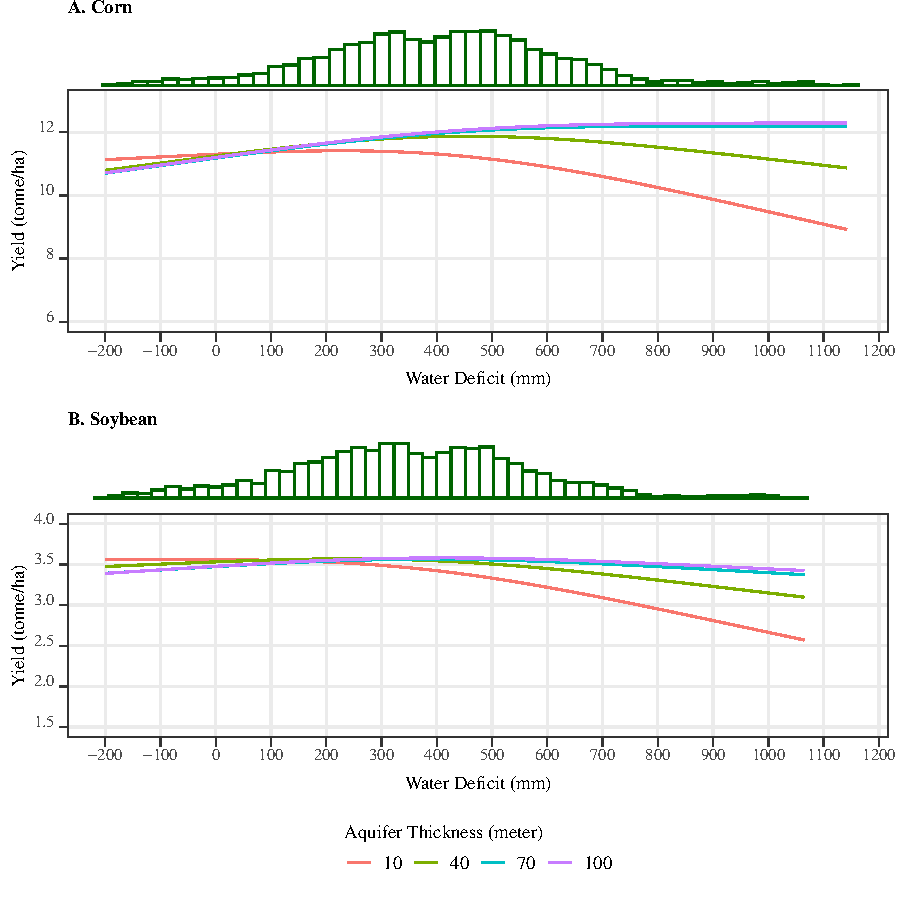
\includegraphics[width=6in,]{Figures/g_total_impact} 

}

\caption{Average productivity of corn and soybean in the US High Plains for different levels of water deficit and aquifer thickness}\label{fig:tot-impact}
\end{figure}

\begin{figure}[H]

{\centering 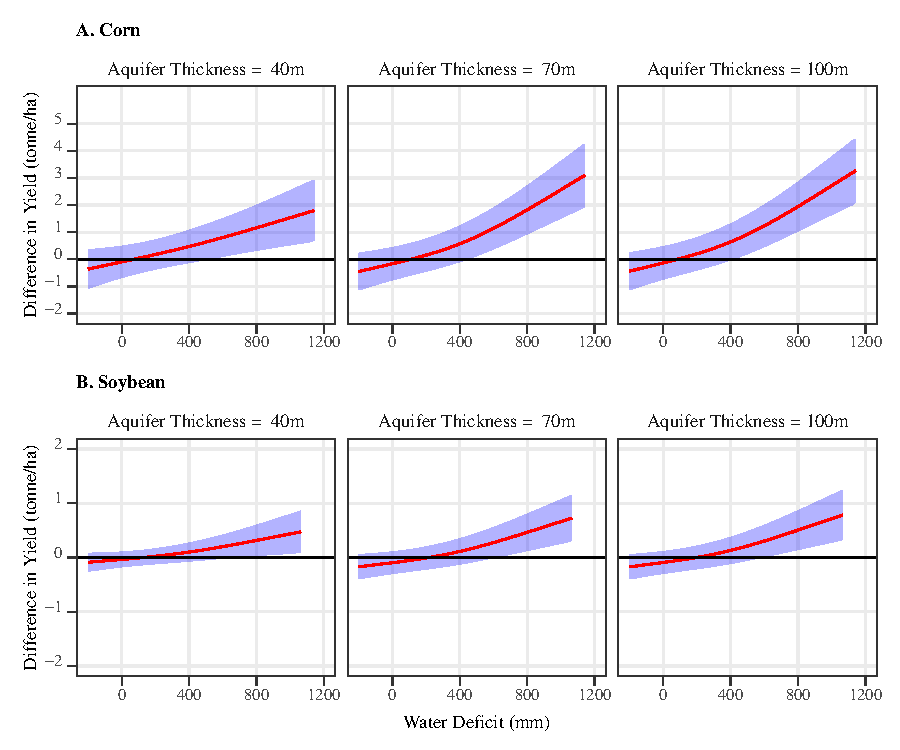
\includegraphics[width=6in,]{Figures/g_avg_yield_dif} 

}

\caption{Difference in average yield relative to the 1st aquifer thickness quantile for corn and soybean}\label{fig:dif-tot-impact}
\end{figure}

\clearpage

\hypertarget{discussion}{%
\section{Discussion}\label{discussion}}

We demonstrate the important role of aquifer thickness in determining farmers ability to successfully buffer crops against drought risks in groundwater irrigated agricultural systems such as the High Plains of the United States. Previous research focused on impacts of drought on agricultural systems has largely focused either on risks for rainfed production \citep{schlenker2009nonlinear, lobell2014greater, schlenker2010robust, zhou2020connections, borgomeo2020impact} or for irrigated lands where water supply constraints are assumed to be minimal \citep{kuwayama2019estimating, zipper2016drought, zhu2022untangling, zhu2022warming, lu2020mapping, davis2019sensitivity, li2018changes, luan2021combined}. Our analysis adds new empirical insights to this literature which show explicitly that reductions in aquifer thickness increase the vulnerability of irrigated agricultural production areas to drought events. Critically, this suggests that commonly adopted binary definitions of agricultural land areas into rainfed and irrigated categories are likely to underestimate exposure of crop production to drought risks, in particular in areas where water supplies for irrigation are insufficient to fully meet crop water needs in all years due to constraints imposed by hydrology, policies, and/or economics.

An important implication of our findings is that depletion of groundwater resources is likely to increase significantly the vulnerability of agricultural production to current and future drought risks. Climate change is projected to increase the frequency and severity of extreme drought events in many parts of the world \citep{ukkola2020robust, chiang2021evidence, cook2020twenty}, including in parts of Kansas and Texas \citep{bradford2020robust, cook2022projected, mullens2019quantitative} where the High Plains Aquifer continues to experience prolonged and significant declines in aquifer thickness \citep{scanlon2012groundwater, haacker2016water, cotterman2018groundwater}. Similar trends of increasing drought risks coupled with declining aquifer storage have been reported in other major groundwater irrigated farming systems worldwide \citep{wada2010global, doll2014global, famiglietti2014global, feng2018groundwater, bierkens2019non}. Our findings suggest that these simultaneous changes in aquifer conditions will amplify impacts of future climate change on crop production, with associated ramifications for resilience of supply chains, commodity markets, rural economies, and food security.

Our findings also provide useful guidance for water managers and policymakers seeking to address unsustainable groundwater use in the US High Plains and globally. Consistent with prior theoretical modeling, we demonstrate that the relationship between aquifer thickness and drought impacts is highly non-linear when accounting for farmers decisions about irrigated production areas. This indicates that sustainable groundwater conservation efforts \citep{macewan2017hydroecon, butler2020charting, elshall2020groundwater} should be targeted in space and time to avoid depletion exceeding critical thresholds which impair farmers' ability to effectively buffer production against drought. Analysis such as ours can provide valuable evidence about these critical thresholds and tipping points to guide proactive management of groundwater stocks, and, in doing so, limit economically damaging transitions from irrigated to rainfed production \citep{foster2017effects, deines2020transitions}. For example, several groundwater management agencies in the Texas portion of the HPA have in recent years set out targets to ensure 50\% of current aquifer storage remains in 50 years time (so called 50/50 rule) \citep{closas2018chronicle}. The effectiveness of such targets could likely be improved substantially by setting conservation targets based on empirical evidence about the level of aquifer thickness that is required to ensure adequate levels of drought protection, both now and with future climate change.

Several opportunities exist for future research to build upon the methods and analyses presented here. First, due to the limited resolution of our observational data, we were only able to estimate the impacts of different aquifer thickness categories on drought risk. Availability of sub-county crop yield data, for example from satellite remote sensing and/or in-situ monitoring \citep{edreira2020combining, deines2021million}, would allow models of the continuous effect of aquifer thickness on drought risk to be developed. Similarly, unobserved variations in aquifer properties will also introduce noise into the relationships between aquifer thickness, well yields, and drought risk exposure. For example, a thinner aquifer interval composed of coarse sands and gravels may be able to supply comparable or higher well yields than a thicker aquifer dominated by fine sands and silt deposits, and hence offer greater resilience to drought despite similar or larger aquifer thickness \citep{butler2013interpretation, korus2020depletion}. While we identify statistically robust impacts of aquifer thickness on drought risk despite these uncertainties, improved data on spatial variations in aquifer properties and greater monitoring of real-world changes in well capacities alongside traditional water level measurements would help to refine understanding of patterns of drought vulnerability across the HPA. This would enable more precise estimates to be made of critical tipping points in the resilience of irrigated agriculture to drought, which are needed to effectively design and target groundwater conservation policies.

Second, our analysis considered the effects of aquifer thickness on farmers decisions to switch from irrigated to rainfed production, but did not assess other potential responses to aquifer depletion such as changing crop types. Switching to more drought resistant crops or varieties may enable farmers to maintain irrigated production at lower levels of aquifer thickness, and has been shown to be an important response to increasing agricultural water scarcity and abstraction policies in other studies \citep{bhattarai2021impact, deines2019quantifying, manning2017producer}. Improvements to irrigation scheduling and water management practices, such as have been implemented as part of the SD6-LEMA (Local Enhanced Management Area) in Kansas \citep{deines2019quantifying, glose2022quantifying} and proposed as part of California's SGMA (Sustainable Groundwater Management Act) \citep{berbel2019droughts, lubell2020sustainable}, could also play an important role in improving the efficiency of irrigation and, hence, the ability to more effectively meet crop water demands with lower well capacities. These kinds of interventions would be likely to reduce - but not eliminate - the increases in drought risk caused by declining aquifer thickness, and could bring additional benefits of reducing over-use of water in wetter years through greater awareness of efficiency saving potentials \citep{foster2019assessing} and the importance of conservation \citep{marston2022} amongst growers. Future research should therefore explore potential strategies that farmers could adopt to lessen the combined impacts of drought and aquifer depletion, alongside efforts to curb unsustainable groundwater extraction and climate change.

Finally, we focus on the impacts of aquifer thickness on agricultural resilience to seasonal water deficits. However, where water deficits are distributed unevenly during the season, negative impacts of aquifer depletion may be even larger. This is because reductions in well yields caused by aquifer depletion will constrain farmers ability to meet peak crop water demands, increasing yield losses compared with if water deficits had been distributed evenly throughout the season \citep{ortiz2019unpacking}. Furthermore, irrigation also has broader benefits for crops such as reducing heat-related stress through cooling of land surface temperatures \citep{adegoke2003impact, bonfils2007empirical, lobell2008effect, zhu2022untangling}. Reductions in aquifer thickness therefore may have other negative impacts on irrigated crop productivity, if constraints to water supply due to aquifer depletion are significant enough to limit cooling benefits of irrigation during the growing season.

\hypertarget{methods}{%
\section{Methods}\label{methods}}

\hypertarget{data-sets}{%
\subsection{Data-sets}\label{data-sets}}

Our study focuses on the High Plains Aquifer (HPA) in the Central United States. Irrigated agriculture is central to the landscape and economy of the High Plains Aquifer, with the region accounting for the majority of grain production in the United States valued in the billions of dollars annually \citep[ \citet{smidt2016complex}]{fenichel2016measuring}. To evaluate the impacts of aquifer depletion on agricultural production overlying the HPA, we rely on data from several sources, which are described below.

County-level irrigated and rainfed yield data for corn and soybean for 1985 through 2016 were obtained from the U.S. Department of Agriculture's National Agricultural Statistics Service (USDA-NASS). USDA-NASS does not report irrigated yields disaggregated by the source of water used for irrigation. However, it is known that groundwater is the main source of water for irrigation for counties that overlie the HPA due to the limited availability of surface water resources in this area. Therefore, we retain both rainfed and irrigated yield observations for counties where greater than 75\% of the county area overlies the boundary of the HPA. For counties that do not meet this condition, only rainfed yield observations are obtained to avoid the possibility that irrigated production may be only partly dependent on use of groundwater from the HPA. We also include additional rainfed yield observations for counties that are outside the HPA, but within the main states covering the aquifer (i.e., South Dakota, Wyoming, Colorado, New Mexico, Nebraska, Kansas, and Texas), to enable more accurate estimation of the impact of drought for rainfed production.

Meteorological data needed to estimate spatial and temporal variations in drought conditions across the HPA were obtained from the gridMET dataset \citep{Abatzoglou2013}. The gridMET data is a gridded daily weather dataset with a spatial resolution of \textasciitilde4km, and has been used in a range of climate impacts studies for agriculture and other sectors in the United States \citep{abatzoglou2016impact, pereira2015crop, crane2018machine, venkatappa2021impacts, zhu2019dissecting}. Daily precipitation values were extracted for each gridMET cell overlapping counties in our sample. Daily values of maximum and minimum temperature, surface radiation, wind speed, and humidity were also obtained from gridMET, and were then used to calculate daily reference crop evapotranspiration for each grid cell. From these data, we computed the seasonal water deficit (\(WB_{i,t}\)) for each grid cell by subtracting total precipitation from total reference evapotranspiration for the period May through September, which represents the typical growing season for corn and soybean in the HPA region. Seasonal water balance estimates were subsequently aggregated to the county-level to match our agricultural production data using an area-weighted average based on the proportion of the county covered by each overlapping gridMET cell. Figure \ref{fig:deficit-yield-hist} presents annual water deficit by year for the corn and soybean data, illustrating major drought events in the region in years such as 2000, 2002, and 2012. The importance of irrigation is clearly evident in these extreme drought years, with rainfed yields dipping substantially whereas irrigated yields are mostly unaffected (Figure \ref{fig:deficit-yield-hist}).

\begin{figure}[H]

{\centering 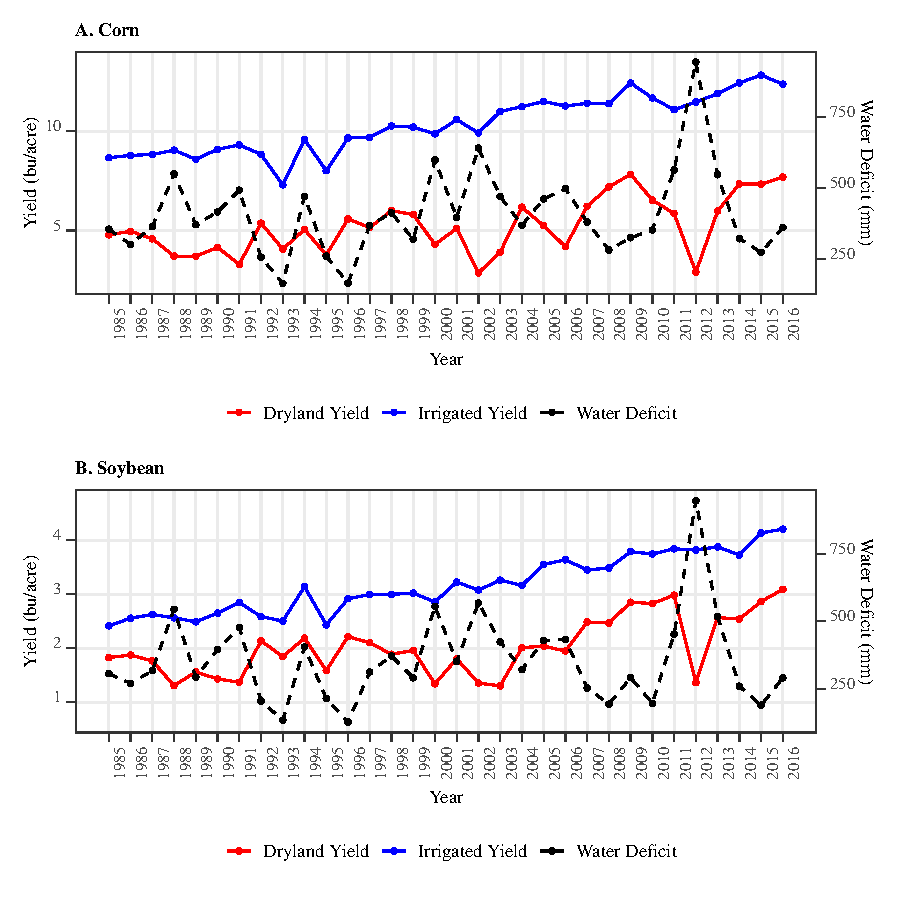
\includegraphics[height=6in,]{Figures/g_y_wd_all} 

}

\caption{Historical dryland yield, irrigated yield, and water deficit}\label{fig:deficit-yield-hist}
\end{figure}

As a proxy for the extent of aquifer depletion we use annual estimates of aquifer thickness for the HPA available at Hydroshare \citep{haacker2023}. These data provide annual estimates of the aquifer thickness of the aquifer at 250m resolution since 1935, derived based on extensive water level observations from monitoring wells and detailed maps of both land surface elevation and the bedrock elevation of the HPA. aquifer thickness estimates for each year were aggregated to the county level using an area-weighted average to match the resolution of agricultural production data. aquifer thickness values were only estimated for counties with irrigated yield observations. Furthermore, during the aggregation process, any aquifer cells within a county that had a aquifer thickness value lower than 12m were removed before aggregation to reflect the fact that aquifer thickness lower than this threshold are not considered to be viable for extraction and therefore it is unlikely these areas contribute groundwater for irrigation production \citep{fenichel2016measuring, haacker2016water, deines2020transitions}. Figure \ref{fig:sat-map} presents the distribution of aquifer thickness across our study area for counties included in corn and soybean analyses. aquifer thickness levels vary substantially over space and time, which we will exploit in our analysis to quantify how aquifer influences farmers' exposure and responses to drought.

These data were combined to form four sets of data for regression analysis: (1) per-acre corn yield (8773 observations), (2) per-acre soybean yield (5977 observations), (3) share of irrigated corn (2686 observations), and (4) share of irrigated soybean (2014 observations).

\begin{figure}[H]

{\centering 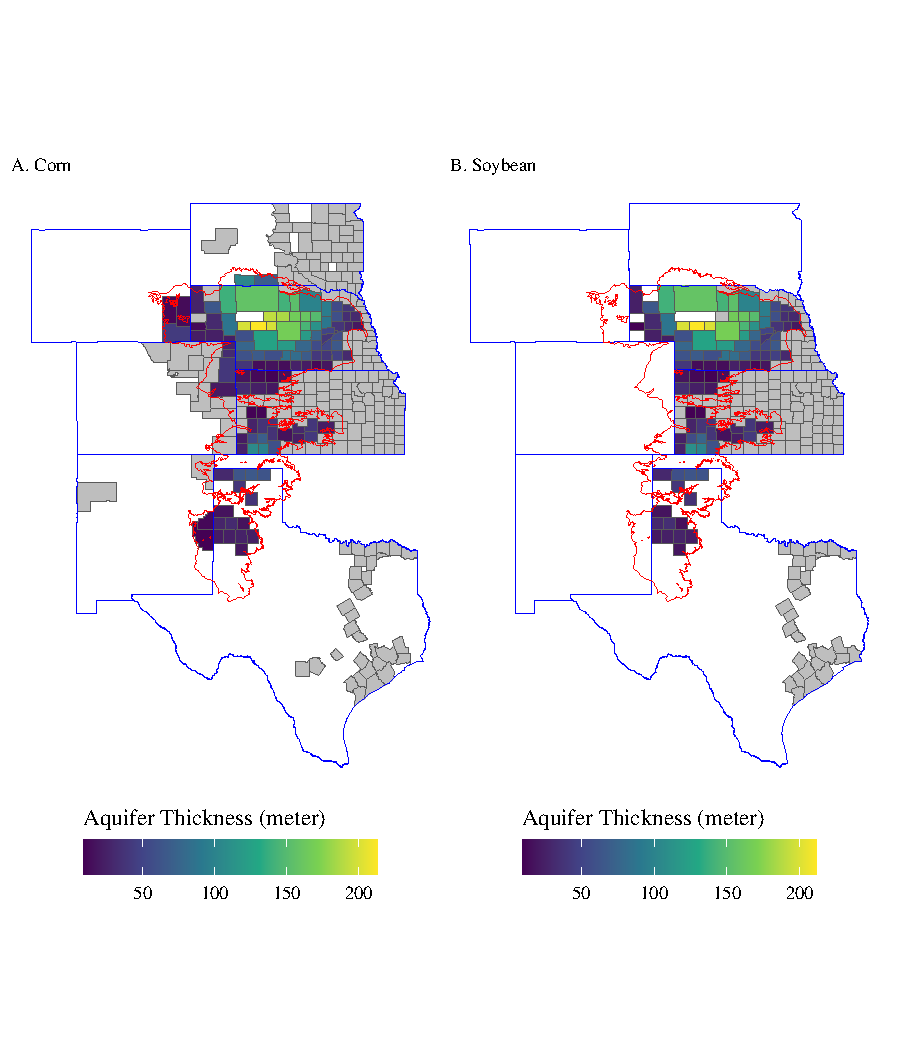
\includegraphics[width=6in,]{Figures/g_map} 

}

\caption{Map showing aquifer thickness in 2016 for each county included in our corn and soybean regression analyses. Counties highlighted in grey are rainfed only, and the red polygon denotes the boundary of the High Plains Aquifer system}\label{fig:sat-map}
\end{figure}

\hypertarget{regression-models}{%
\subsection{Regression Models}\label{regression-models}}

Aquifer depletion may impact resilience of irrigated crop production to drought through two main channels: (1) a reduction in per-area irrigated yields due to the economic or physical inability to meet crop water requirements; and (2) a reduction in the area of land irrigated, resulting in reduced production due to lower yields obtained through rainfed agriculture.

To assess the first of these impacts, we quantify the impact of seasonal water deficits (\(WB\)) during the growing season (May through September) on county-level rainfed and irrigated yields (\(Y\)) using a hierarchical generalized additive model, where irrigated yield to drought is conditioned on the level of aquifer thickness (\(AT\)) in the county in a given year. Our regression model is given in Equation \eqref{eq:eqn1}, with the same model formulation used for corn and soybean:

\begin{equation}
y_{i,t} = \sum_{j=1}^4 \sigma_j C_j + \sum_{j=1}^4 \sum_{k}^K \beta_{j,k}\phi_{j,k}(WB_{i,t})\cdot C_j  + \alpha_i + \phi_t + v_{i,t} \label{eq:eqn1}
\end{equation}

where county and year are indicated by subscripts \(i\) and \(t\), respectively, \(y\) is crop yield, and \(WB\) is seasonal water deficit. \(C_j\) is a dummy variable that takes 1 if observation \(i\) is under category \(C_j\), 0 otherwise. The observations are grouped into four categories: rainfed production, and county-years with aquifer thickness falling in the \([0-33.3\%)\), \([33.3-66.7\%)\), and \([66.7\% - 100\%]\) quantile ranges of aquifer thickness. The three irrigated production groups have about the same number of observations, which ensures statistical stability in estimating yield response to drought by category. Spline functions are used to capture the potential non-linearity of the impact of water deficit on yield in a flexible manner, with \(\sigma_j\) represents the category specific intercept, \(\phi_{j,k}\) \(k\)th spline basis function, and \(\beta_k\) is its coefficient (see Appendix \ref{spline-basis} for further explanations on how spline-based regression works). To control for time-invariant heterogeneity across counties and yearly shocks, county fixed effects (\(\alpha_i\)) and year fixed effects (\(\phi_t\)) are also included and standard error estimation is clustered by county.

To estimate the additional impact of aquifer thickness on the share of total acres that are irrigated in a county, a fractional logit model under the generalized additive model framework is used in which the impact of aquifer thickness, average water deficit, and their interactions are estimated without needing to assume any functional forms. This allows for flexible representation of the non-linear relationships between drought risks, aquifer conditions, and agricultural land use, including potential thresholds in farmers irrigated area choices under water supply constraints that have been noted in prior work \citep{foster2015well, foster2015analysis, hrozencik2017heterogeneous}. The model is given in Equation \eqref{eq:eqn2} below:

\begin{equation}
    log(\frac{s_{i,t}}{1-s_{i,t}}) = \beta_0 + \sum_{k}^K \alpha_{k}\phi_{k}(WB_{i}) + \sum_{l}^L \beta_{l}\tau_{l}(AT_{i,t}) + X_i + \theta_{s,t} + \mu_t + v_{i,t} \label{eq:eqn2}
\end{equation}

where \(s_{i,t}\) is the share of irrigated production. The impact of average water balance is captured by \(\sum_{k}^K \alpha_{k}\phi_{k}(WB_{i})\), where \(\phi_{k}(\cdot)\) is the \(k\)th spline basis function and \(\alpha_{k}\) is its coefficient. The impact of aquifer thickness is captured in a similar way with \(\tau_{l}(\cdot)\) and \(\beta_{l}\) being the \(l\)th spline basis function and its coefficient, respectively. County-level soil characteristics including sand percentage, silt percentage, and water holding capacity, are represented by \(X_i\). State-year fixed effects and error term are represented by \(\theta_{s,t}\) and \(v_{i,t}\), respectively. One of the limitations here is that we do not include county fixed effects to avoid eliminating the majority of variation in the aquifer thickness variable unlike our regression model of the impact of water balance on yield. The vast majority of variation in aquifer thickness is cross-sectional (across counties), rather than over time. Including county fixed effects effectively eliminate the cross-sectional variation in aquifer thickness. The trade-off here is tighter controls on potential unobservables that may be correlated with aquifer thickness (see Appendix \ref{county-fe} for more discussions).

In the final step of our analysis, we then estimate the average crop yield as a function of aquifer thickness and seasonal water deficit. The average crop yield is estimated as the average of rainfed and irrigated yields estimated on the basis of Equation \eqref{eq:eqn1}, weighted by the estimated share of total acres that are irrigated in the county estimated using Equation \eqref{eq:eqn2}. Comparing the estimated average crop yield across different levels of aquifer thickness for a given seasonal water deficit provides an indication of the effect of aquifer conditions on drought impacts, considering impacts of drought through changes in both per-area irrigated yields and the area of land irrigated. Its standard error is estimated using bootstrap clustered by county.

\hypertarget{data-and-code-availability}{%
\subsection{Data and Code Availability}\label{data-and-code-availability}}

All the codes used for this study are available at the following Github repository (\href{https://github.com/tmieno2/Drought-Production-Risk-Aquifer}{link}). All the computations were done in R \citep{R} and all the raw data-sets used in this study are publicly accessible. The boundary shape file of the High Plains aquifer was obtained from the U.S. Geological Survey at \url{https://water.usgs.gov/GIS/metadata/usgswrd/XML/ds543.xml#stdorder}. This data is used for Figure \ref{fig:sat-map}. Corn and soybean yield data were obtained from the U.S. Department of Agriculture's National Agricultural Statistics Service (USDA-NASS), available at \url{https://www.nass.usda.gov/Quick_Stats/}. The R tidyUSDA package \citep{RtidyUSDA} was used to automatically download the relevant data. This data is used for Figure \ref{fig:deficit-yield-hist} and the regression analysis. Weather data (precipitation, temperature, and evapotranspiration) was obtained from the gridMET dataset \citep{Abatzoglou2013}, which is available at \url{https://www.climatologylab.org/gridmet.html}. This data is used for Figure \ref{fig:deficit-yield-hist} and the regression analysis. The aquifer thickness data were obtained from Hydroshare \citep{haacker2023}. This data is used for Figure \ref{fig:sat-map} and the regression analysis. Soil characteristics data was obtained from the Soil Survey Geographic Dataset, which is used for regression analysis. The R soilDB package \citep{Rsoildb} was used to download the data. Regression analyses are implemented using the R fixest package \citep{Rfixest}. Other key R packages include ggplot2 \citep{Rggplot2} for creating plots, data.table \citep{Rdatatable} for data wrangling, and sf \citep{Rsf} for spatial data operations. The data used for the regression analysis can be generated using our codes by following the instruction available at the Github repository.

\clearpage

\hypertarget{appendix-appendix}{%
\appendix}


\hypertarget{reg-conf}{%
\section{More on the impact of water deficit on irrigated and average yield}\label{reg-conf}}

\setcounter{figure}{0}
\renewcommand{\thefigure}{A.\arabic{figure}}

In the main article, the confidence intervals of the estimated yield responses to water deficit were not presented as they would crowd the figures excessively. This section provides visualization of yield response with the 95 \(\%\) confidence interval to convey the degree of uncertainty in our estimation. Figures \ref{fig:irrigated-yield-ind-corn} and \ref{fig:irrigated-yield-ind-soy} present the impact of water deficit on crop yield by aquifer thickness category with the 95\(\%\) confidence interval for irrigated corn and soybean, respectively. Figure \ref{fig:avg-yield-ind} presents the impact of water deficit on average crop yield (irrigated and rainfed combined) by aquifer thickness category for corn and soybean with the 95\(\%\) confidence interval.

\begin{figure}[H]

{\centering 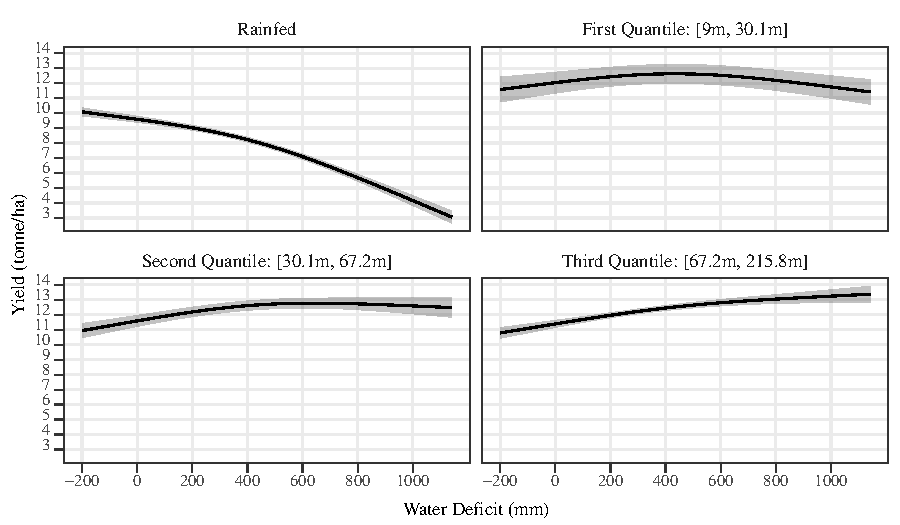
\includegraphics[width=6in,]{Figures/g_yield_with_conf_corn} 

}

\caption{The impact of water deficit and aquifer thickness on rainfed and irrigated per-area irrigated yields of corn in US High Plains with 95 percent confidence interval}\label{fig:irrigated-yield-ind-corn}
\end{figure}

\begin{figure}[H]

{\centering 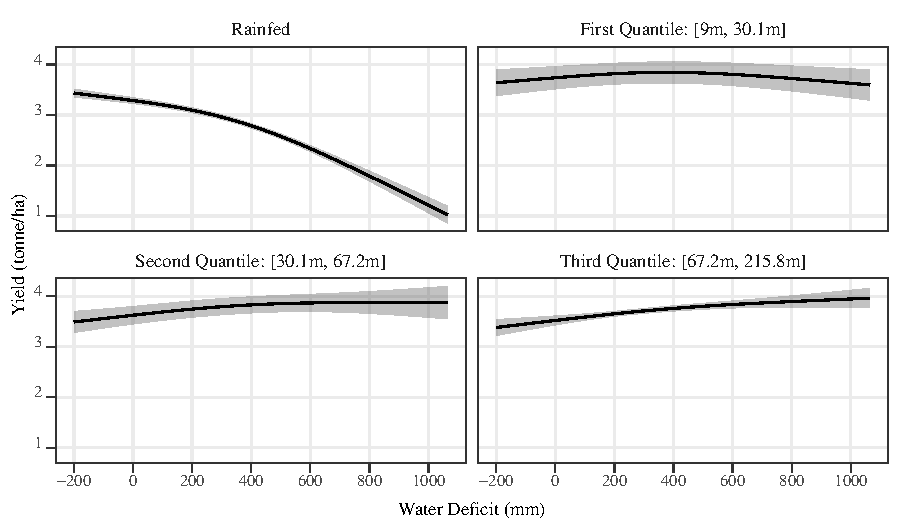
\includegraphics[width=6in,]{Figures/g_yield_with_conf_soy} 

}

\caption{The impact of water deficit and aquifer thickness on rainfed and irrigated per-area irrigated yields of soybean in US High Plains with 95 percent confidence interval}\label{fig:irrigated-yield-ind-soy}
\end{figure}

\begin{figure}[H]

{\centering 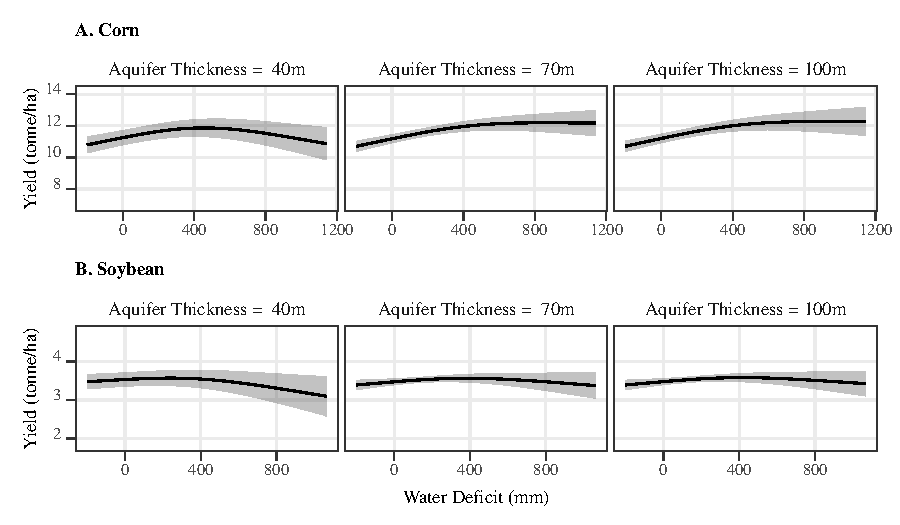
\includegraphics[width=6.5in,]{Figures/g_avg_yield} 

}

\caption{Average productivity of corn and soybean in the US High Plains for different levels of water deficit and aquifer thickness (The shaded areas represent the 95 percent confidence interval)}\label{fig:avg-yield-ind}
\end{figure}

\clearpage

\hypertarget{county-fe}{%
\section{County Fixed Effects in Irrigation Share Regression}\label{county-fe}}

\setcounter{figure}{0}
\renewcommand{\thefigure}{B.\arabic{figure}}

Figure \ref{fig:variation-left} presents the histogram of aquifer thickness after demeaning them by its overall average (A), state average (B), and county average (C) to gain insights into how much variation for identification is left under no county or state fixed effects (A), state fixed effects (B), and county fixed effects (C). As you can see in the figure, while including state fixed effects do not reduce the total variation in aquifer thickness, including county fixed effects dramatically reduces its total variation. Consequently, we found that including county fixed effects results in extremely inaccurate estimates (high standard error). For this reason, we just included state fixed effects.

\begin{figure}[H]

{\centering 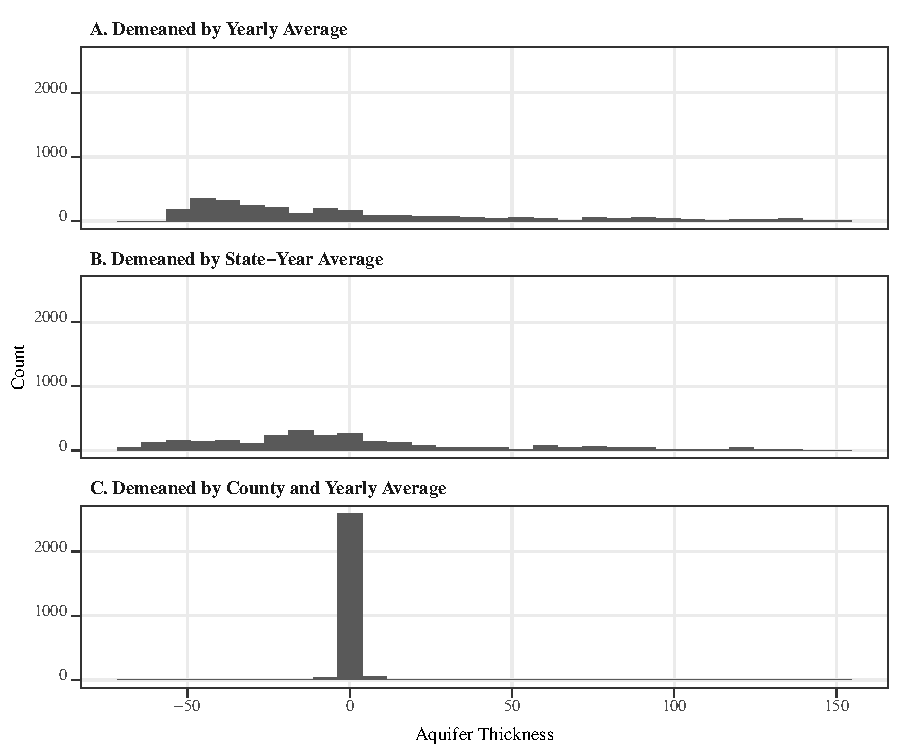
\includegraphics[width=6in,]{Figures/g_variation} 

}

\caption{Comparison of variations in aquifer thikcness after demeaning by overall average, county average, and state average.}\label{fig:variation-left}
\end{figure}

Figure \ref{fig:state-fe-with-without} compares the impact of aquifer thickness on the share of irrigated acres for corn and soybean with different sets of fixed effects. For both corn and soybean, the negative impact of reduction in aquifer thickness on the share of irrigated acres are virtually the same across the sets of fixed effects. Most important, adding state fixed effects, which control for unobservables at the state level, does not change the estimation results much. Therefore, even though there may be unobservables that are spatially correlated with aquifer thickness, their correlation may not be very strong to cause significant bias. Clearly, this does not mean that our inability to control for other county-level unobservables beyond sand percentage, silt percentage, and water holding capacity is not causing bias in our estimation of the impact of aquifer thickness on the share of irrigated acres.

\begin{figure}[H]

{\centering 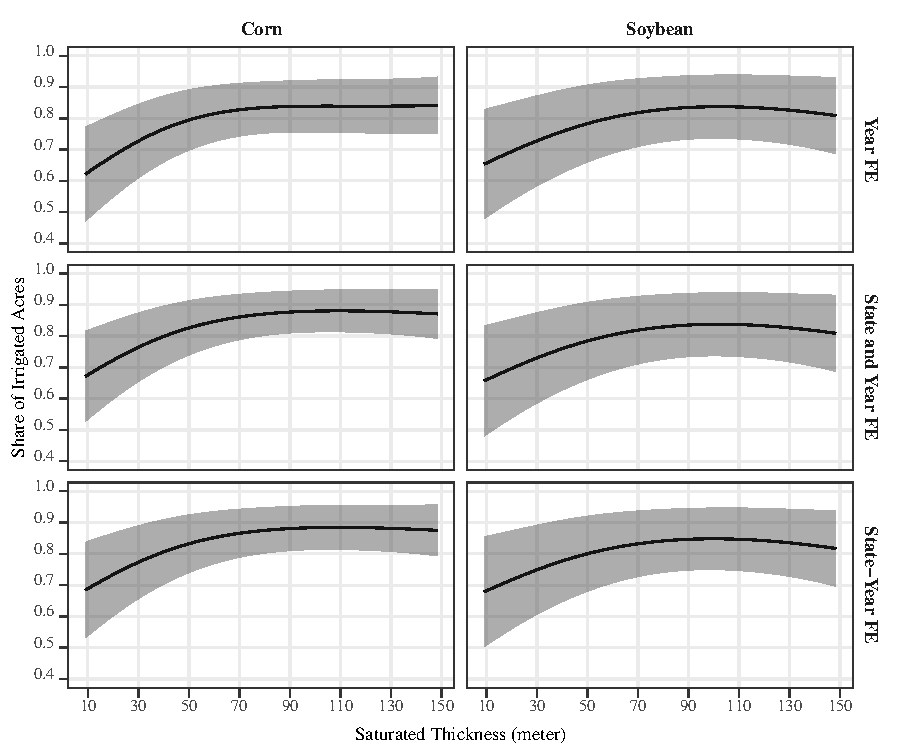
\includegraphics[width=6in,]{Figures/g_share_comp} 

}

\caption{Comparison of estimated impact of aquifer thickness on the share of irrigated acres with and without state fixed effects}\label{fig:state-fe-with-without}
\end{figure}

\clearpage

\hypertarget{spline-basis}{%
\section{Spline basis functions and GAM estimation}\label{spline-basis}}

\setcounter{figure}{0}
\renewcommand{\thefigure}{C.\arabic{figure}}

We used generalized additive models (GAM) for our regression analysis. In GAM, the impact of a variable on the dependent variable can be expressed as a series of spline basis functions and their coefficients. Suppose you are interested in modeling the following model.

\begin{equation}
y = f(x) + \mu
\end{equation}

Where \(f(x)\) represents the impact of variable \(x\) on \(y\). The shape of \(f(x)\) is not known to the researcher. GAM attempts to represent \(f(x)\) with a series of spline basis functions and their coefficients like below.

\begin{equation}
y = \sum_{k=1}^K \beta_k \phi_k(x) + \mu
\end{equation}

Where \(\phi_k(\cdot)\) is the \(k\)th spline basis function and \(\beta_k\) is its coefficient. Figure \ref{fig:sp-basis} provides a visual illustration of a series of thin-plate spline basis functions.

\begin{figure}[H]

{\centering 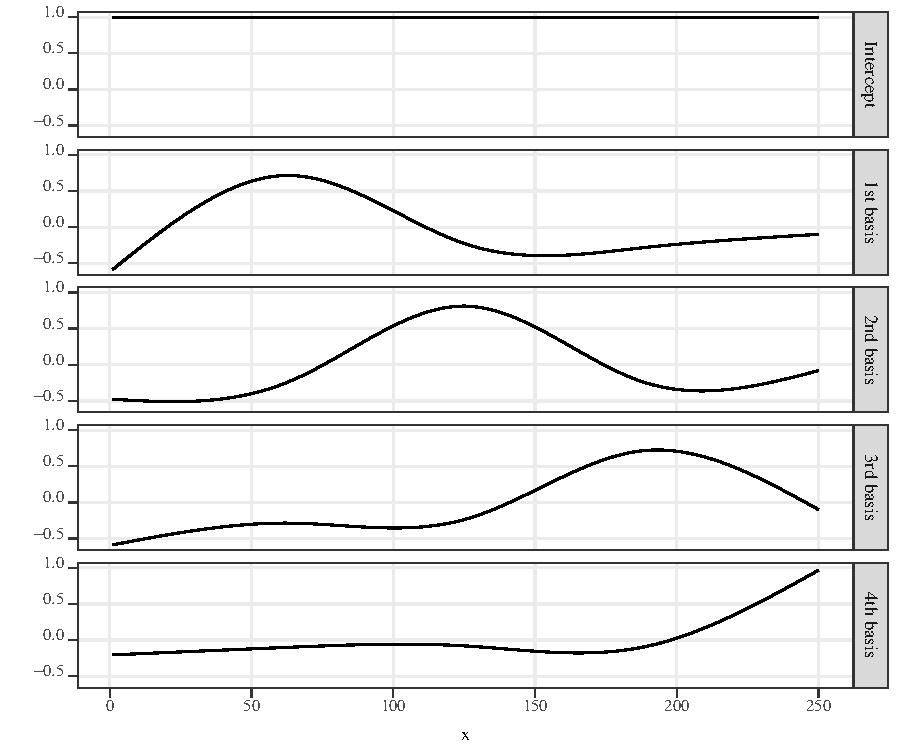
\includegraphics[width=6in,]{Figures/g_basis} 

}

\caption{Example of a series of thin-plate spline basis functions}\label{fig:sp-basis}
\end{figure}

Different coefficients (or namely weights) given to the spline basis functions result in different shapes of the imapact of \(x\) on \(y\). Figure \ref{fig:ex-fx} presents two examples of two different sets of coefficients and their resulting representation of \(f(x)\). In the first case, \(\{\beta_1, \dots, \beta_5\} = \{60, 60, 60, 60, 60\}\). In the second case, \(\{\beta_1, \dots, \beta_5\} = \{20, -20, -40, 40, 60\}\). Among all the possibilities of the combinations of the coefficients, GAM finds the set of coefficient values that fits the data best. Notice that unlike non-parametric regression, GAM is actually a linear in parameter model and estimate \(\beta_k\) to fit the data best.

\begin{figure}[H]

{\centering 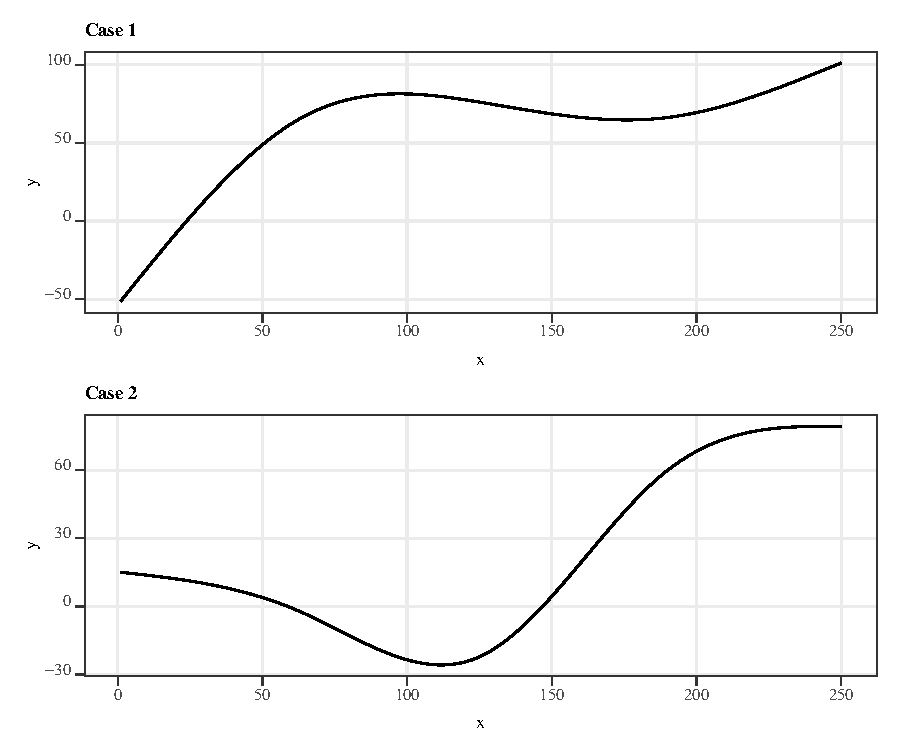
\includegraphics[width=6in,]{Figures/g_il_y} 

}

\caption{Example of a function represented by different coefficient values}\label{fig:ex-fx}
\end{figure}

\clearpage

  \bibliography{DRA.bib}

\end{document}
